\graphicspath{{two-routes-estimation/}}

\chapter{Two Routes to Improved Numerical Estimates}
\label{chap:two}

As described in Section~\ref{sec:two}, cognition can occur in a relatively local
or special-purpose manner, or alternatively in an integrated fashion that (among
other things) affords volitional or conscious access. In
\cite{clark_known_2010}, we provide some preliminary evidence and argumentation
for separable learning processes which might be differentially involved when
learning numerical information. Below, I present an overview of two experiments
in abbreviated form, noting those details that are relevant to the questions
posed above. Specifically, these results demonstrate our ability to observe, and
potentially guide cognition between heavily conceptual \emph{episodic} or
\emph{semantic} modes of operation on one hand, and less conceptual emotional
processing on the other.

\section{Overview}

In short, participants saw textual descriptions of numeric items and provided
their best estimate. After this, they received the true value, and indicated the
degree to which they found the true value \emph{surprising}. After a period
including at least one night's sleep, participants were presented with the
previously shown textual descriptions.  Here, participants indicated their
\emph{metacognitive assessment of their memory} from the item from the day
before, in addition to re-estimating (or potentially recalling) the value.

\section{Experimental Methods}

The following experiment was designed to assess whether estimative improvement
occurs even with respect to items for which no feedback was received---as was
found in curricular NDI studies
\cite[e.g.,][]{munnich_numerically-driven_2004,ranney_designing_2008}. The
experiment (1) addresses the effects of surprise and the timing of feedback on
subsequent improvements in numerical estimation---as well as (2) probes whether
these improvements are necessarily mediated by explicit recollection. A subset
of the EPIC procedure was used to explore these issues; participants engaged
only in estimation (``E'') and feedback (``I''), leaving aside personal
preference (``P'' and ``C''). 

\subsection{Participants}

Twelve people (seven female) participated, including UC Berkeley undergraduates
and members of the general public recruited via online recruitment systems (RPP
and RSVP). They received either course credit or \$20 for their participation in
two one-hour sessions over two consecutive days. Ages ranged from 18-56 years. 

\subsection{Materials}

Numerical facts (106 of them) were selected from \citeauthor{ranney_designing_2008}
. An example is ``The current percentage of deaths in the U.S. that are
caused by lung cancer.'' Three statistical facts were set aside for the basis of
example items (namely US population, world population, and US Gross National
Income). Items ranged over a number of topics, and included politics, population
dynamics, economics, the environment, education, crime etc. Most items were
expressed in percentage form, with the rest being counts of dollars, people,
events or things. For numbers above 999, a comma was used, as in ``13,600.''  For
numbers in the millions, billions, or trillions, the appropriate word was used
to indicate the order of magnitude (e.g., ``300 million'').  This was intended to
minimize possible confusions about the exact value of the number.

\subsection{Procedure}

Custom software utilizing Vision Egg \cite{straw_vision_2008} presented all materials and
collected responses. (Source code available upon request,)  Descriptions of
numerical facts were presented in 1-4 lines of text (with less than 55
characters per line). A prompt for numeric entry was located below the
description. Feedback concerning the veridical value was provided in a third
location, between the description and the text-entry area.

\subsubsection{Blocks of Items}

Items were randomly distributed into the following four kinds of blocks. Each of
these blocks was involved in two or more runs over the course of the experiment.
E: Participants only provided Estimates in a single run. EI: Participants
provided Estimates followed immediately by correct numerical Information as
feedback (i.e., feedback was provided in the same run as the initial
estimation). E\_I: Participants provided Estimates, then received correct
numerical Information in a run that was well-separated from the run in which
they provided their Estimate (i.e., ``\_'' signifies a temporal delay). New: A
block of items was reserved in both experiments to provide a gauge of false
recognition or false recollection.

\subsubsection{Experimental Runs}

Participants engaged in a number of self-paced runs on each of the two
consecutive days, as figure~\ref{ei-procedure} depicts. The presentation of
stimuli and responses made were uniform across a given run. During the first
day, analogous to a ``study'' phase, participants completed three partially
similar runs of numerical estimation and/or informative feedback. The second day
was analogous to a ``test'' phase, in which participants’ learning was assessed.

 
%% This probably doesn't go here
\begin{figure}[h]
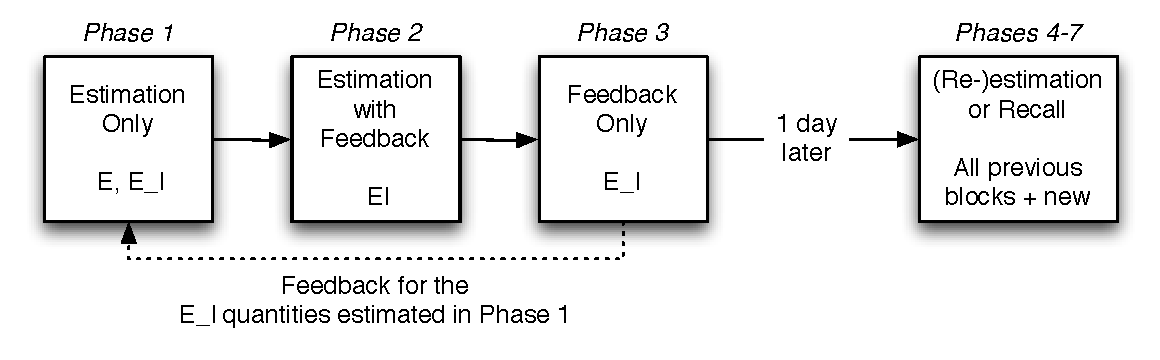
\includegraphics[width=\textwidth]{Experiment1-procedure.pdf}
\caption{A schematic of the experiment's seven runs. Run 1:
Estimates were obtained for the E and E\_I blocks of items (23 each), randomly
intermixed in one run. Run 2: Participants provided 23 Estimates that were
immediately followed by Informing the participant of the correct value. Run 3:
Feedback (I) was provided for the 23 items from the E\_I block that had been
Estimated in Run 1. Runs 4-7: Subjects estimated (or recalled) quantities and
provided explicit memory ratings for all previous items as well as 34 new
items.}
\label{ei-procedure} 
\end{figure}

During estimation (Runs 1 and 2, with 23 items each), subjects were given a
textual description of an item's quantity, followed by a prompt to provide an
estimate. For Run 2, feedback was provided 500 milliseconds after each estimate
was entered. For Run 3 (with 23 items), the correct numerical value was provided
prior to the textual description in order to minimize covert estimation.

In Runs 2 and 3 (thus, for blocks including ``I''), surprise ratings were elicited
regarding the values given as feedback. Three possible levels of surprise were
collected: 

\begin{enumerate}
\item Little or no surprise
\item Genuine surprise
\item ``Visceral'' or intense surprise
\end{enumerate}

On day 2, trials were similar to the estimation-only trials in Run 1 described
above---no additional feedback was provided. An additional 34 items from the
``new'' block were randomly intermixed with the items presented during study.
Additionally, participants rated their memory for the item according to the
following 4 levels: 

\begin{enumerate}
\item ``The item is new to me'' 
\item ``The item was presented yesterday, but I have no sense of the value 
provided as feedback'' 
\item ``The item was presented yesterday, and I have some sense of the correct value''
\item ``The item was presented yesterday, and I have a fairly accurate recollection of
the value.'' 
\end{enumerate}

Choice 1 indicates no recognition or recollection.  This is equivalent to
labeling the item as ``new,'' and it is the correct response for items from the
new block.  Choices 2-4 as a group indicate that the item is ``old,'' but with
varying levels of familiarity and/or recall.  These are correct responses for
the E, EI and E\_I blocks (although choices 3 and 4 entail a belief that the
participant actually received feedback at study, and so might also be considered
incorrect for the E block). Choices 2 and 3 indicate perceived recognition, but
at least a partial failure in recall.  Choice 4 indicates a subjective sense of
fairly complete recall.

Note that the estimation task used here is somewhat different than item
recognition or cued recall tasks used in many learning and memory studies. The
closest point of comparison is likely the notion of \emph{source} memory, in
which details surrounding the initial experience of the experimental item are
well correlated with hippocampal activity at encoding
\cite{davachi_multiple_2003}. In particular, we are \emph{not} asking
participants to attempt to recall a particular item from memory, Indeed, these
memory ratings can be viewed as a form of metacognition regarding the estimation
process and it's relationship to the participants previous experience with the
item (i.e., source memory for the item).

\subsection{Analysis}

We modeled improvement as a binomial outcome \cite[as
did]{munnich_longevities_2005}. This allows for the treatment of items that have
differing distributions within a unified framework (e.g., a linear model would
have difficulty modeling both percentages and values in the billions,
particularly given our sample size).  Items were labeled as to whether estimates
improved or not. These labels were fit with a binomial generalized linear model,
using the lme4 package in the R statistical environment
\cite{r_development_core_team_r:_2009_fixed}. This treatment allows for a full
multi-factorial mixed-effects analysis. Below, participants are always included
as a random effect, and other factors are treated as fixed effects. Linear
contrasts were evaluated using the multcomp package, which controls for
family-wise error rate \cite{hothorn_simultaneous_2008}.

Unless otherwise noted, data were pre-processed to remove ties. This was done to
allow for a null hypothesis that 50\% of the remaining items randomly improved
and 50\% randomly worsened. If we counted ties as failures to improve, then
random drift would end up spuriously suggesting the lack of an effect. Removing
ties allowed for tests of whether estimates improved, on average, more than they
worsened––both formally and when examining graphs. Otherwise, the removal had
little effect on the results, except where explicitly noted below.

%% Include a simplified figure for experimental design
% I need to redo these results (using Sweave) and carefully explain which items
% were excluded

\section{Results}

\subsection{Improvements in Accuracy of Estimation}

We can easily reject a null model in favor of a model predicting different
improvements across ``I,'' ``EI,'' and ``E\_I'' feedback conditions ($\chi^2(2)
= 25.9, p < 10^{-6}$). Post-hoc comparisons between each condition and chance
levels, as well as between condition comparisons (as in a Tukey HSD test) were
performed simultaneously. 
% For this document, it would be good to give the full explanation including
% lme4, glht, etc.
In the no-feedback case (E), estimation improvement
did not differ significantly from chance ($p = 0.39$), although improvement with
Immediate (EI) and Delayed (E\_I) feedback were clearly above chance ($p <
10^{-4}$). This may seem unsurprising, but it might have been the case that
improvements were at least partially driven by general improvements in
estimation skill, and this would have led to at least some modest improvements
even without feedback on test items. Indeed, this kind of skill development was
the successfully accomplished goal of various EPIC-based curricula
\cite[e.g.,][]{munnich_numerically-driven_2004,ranney_designing_2008}. In this
less extensive experimental manipulation, though, we understandably elicit no
such skill improvements. Thus, we assume that these improvements are driven
almost entirely by item-specific learning.

\subsection{Predicting learning from surprise and meta-cognitive memory
assessment}

As is often the case, the participants' forced familiarity judgments appeared to
be superior to their own assessment of their memory.  In participant
debriefings, several individuals claimed to be uncertain whether items were old
even from Run 1 to Run 3 for items in the E\_I block––that is, over an interval
of less than 30 minutes!  However, participants were excellent at discriminating
between old and new items a day later when given a forced choice; 76\% of new
items were identified as new on Day 2, compared to an average of less than 9\%
regarding previously seen items. This level of recognition accuracy is not
surprising given the considerable depth of processing involved, and the rich
pre-existing memory structures available for scaffolding these episodes.

\begin{figure}[h]
\centering
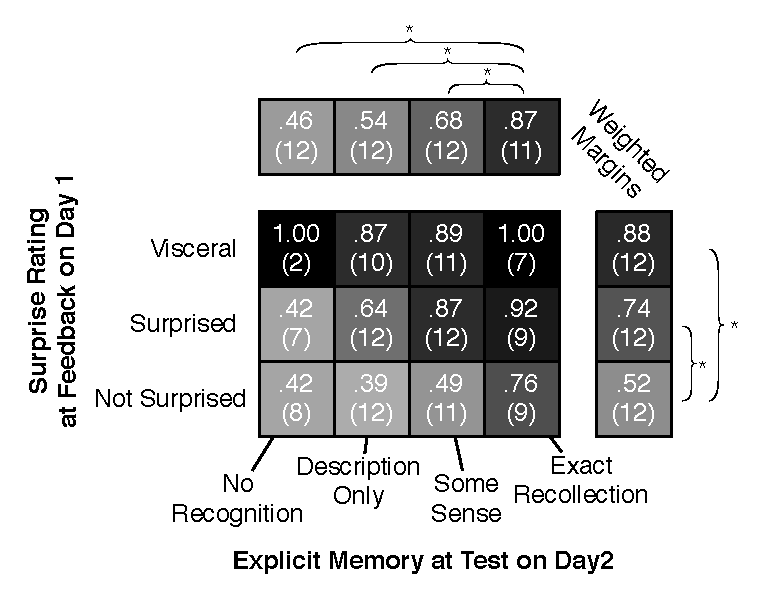
\includegraphics{shaded-table-reversals.pdf}
\caption{Fraction of items improving across different levels of surprise rating
and metacognitive memory assessment. The number is parentheses represents the
number of subjects (out of 12) contributing to that cell. Margins are
appropriately weighted according to the number of items in each bin, and as such
are not the simple mean of the row or column in the central table. Significant
differences between levels of individual factors are marked with an asterisk.}
\label{ei-table} 
\end{figure}

As the lack of feedback yielded non-significant changes in estimation accuracy,
here, we consider only items from conditions including feedback (``I''). These
effects are depicted in Figure 3.  A model that predicts estimation improvements
on the basis of both surprise and declarative memory responses is well-supported
by the data. We readily reject a reduced model excluding memory ($\chi^2(3) =
34.8, p < 10^{-7}$), as well as one excluding surprise ($\chi^2(2) = 295.22, p <
10^{-16}$). An inclusion of an interaction term does not yield a significantly
better model ($\chi^2(6) = 2.85, p = 0.8$). 

% Test for this is in surprise.diff.by.condition function in pilot2 dir
It should be noted, that there is a small (but non-significant)
difference in surprise ratings between EI and E\_I blocks: subjects rated 64\%
of EI block items as surprising (``2'' or ``3'') vs. 59\% for E\_I (although no
straightforward effect was observed with metacognition on memory).  This result
mirrors the result obtained in the above study on climate change cognition, in
which prior estimation increased participant reports of surprise
\cite[cf.][]{rinne_estimation_2006}.  Thus, the
timing of feedback may have an effect on estimation improvement that is mediated
by surprise; these issues seem best addressed in a subsequent study, though.
Below, we only consider comparisons within surprise level and memory ratings
independent from one another.

Recall of the exact value (memory response ``4'') as compared to other memory was
a highly significant predictor of improved estimation (all $p$'s $< 0.001$ for the
lower two ratings, $p = 0.01$ when compared with response ``3''). No other
comparisons between memory levels are significant. For surprise, both moderate
and visceral ratings yielded significantly greater improvement than for
no-surprise rated items ($p < 0.002$ in both cases), but did not differ
significantly from one another. Note that participants provided the exact
numerical figure given as feedback only 35\% of the time when selecting choice
4. Even if we broaden this liberally to items where participants are within 15\%
of the true value, they were only correct about 74\% of the time.

Finally, if we consider the relation between surprise and metacognition on
memory, there
appears to be very little correlation. The correlation of fixed effects between
memory and surprise terms in our model was consistently smaller in magnitude
than 0.1. This, combined with the lack of significance of an interaction term,
provides some evidence for independent learning processes.

While both \emph{surprise} and \emph{metacognitive memory assessment} were
predictive of improved estimation from the first to the second session, these
measures did not interact significantly, and moreover were uncorrelated with one
another (i.e., progressive darkening from the lower-left to upper-right corner
in Fig.~\ref{ei-table}).

%% I have re-run correlations between surprise and metacognition using
%% tetrachoric methods. Looking at the data though, it seems that I should
%% probably employ something like a chi-squared model. I suspect the rows do NOT
%% have identical frequencies, and that visceral surprise does reduce the
%% likelihood of a "new" response

On it's own, this result would be insufficient to make strong claims about
multiple cognitive routes for learning. But, this result fits well with an ever
increasing literature (an overview of which was provided in
section~\ref{sec:two}). 

\subsection{Exclusions}

As many as three items lacked estimates from some subjects or exhibited a clear
lack of understanding (e.g., a number such as 10 million for a question asking
for percentage) and these items were excluded from the analyses above. Due to a
technical issue, participant 01 was not run on the standard E manipulation, but
was included in memory and surprise-related analyses, as these analyses did not
include E trials.

\section{Discussion}

Given the overall improvements in estimation ability evidenced in curricular
studies by \citeauthor{munnich_numerically-driven_2004} and
\citeauthor{ranney_designing_2008}, it is of interest that we see no statistically
significant improvement in items that didn't receive feedback (the ``E'' block).
In other words, it appears that participants did not improve their estimation
skills in the absence of feedback particular to a given item.
Nonetheless, it seems that learning in this considerably shorter experiment was
largely item-specific and related to the integration of feedback. This lack of
improvement in the present experiment may be due to a lack of time for
reflection or development of strategies––which were highlighted, taught, and
fostered in the curricular studies.
(\nptextcite{munnich_numerically-driven_2004,ranney_designing_2008} also focused, to
a fair degree, on preferences and personalized policies which may engage a web
of related concepts.)

\subsection{Learning Without Metacognitive Report of Recall}

From the point of view of a memory theory, the most interesting result is
perhaps the existence of learning even when participants claimed “no sense” of
the numerical value provided at feedback---rather like a memorial analog to
blindsight. This argues against the notion that improvements in estimation are
simply the result of explicit episodic memory. The result is reminiscent of
extant dual-process memory models.  For example, \citeauthor{davachi_multiple_2003}
suggest that successful recognition could occur through a process of
recollection and/or a sense of familiarity.  These processes moreover appear to
be subserved by distinct sub-regions in the medial temporal lobe.  In the
present study, though, we see improvement in numerical estimation---which is
perhaps most akin to a cued recall task for EI and E\_I items---without full
recall of the number presented on the previous day.  Thus, the task here is
perhaps more naturally expressed in the language of the remember/know
distinction \citeauthor{knowlton_relationship_1998}.  That is, while participants
appear not to remember a specific (usually multi-digit) number from the previous
day, there is still a sense in which they know the number better than they knew
it the day before.

Based on the significance of the existing results, however, it seems reasonable
to posit that a non-episodic form of learning undergirds some of the improvement
in participants’ abilities to estimate accurately.  Further, the learning for
improved estimation (or memory) seems to occur often without an explicit, precise
recollection of the feedback from the prior day.  This argues for some implicit
and/or rapidly semanticized learning in support of these improvements. In
particular, this appears to have something of a ``less conceptual'' flavor.
This line of reasoning is reminiscent of studies of children applying abstract
mathematical rules before they are aware of doing so
\cite{siegler_unconscious_2000}.

Of course there is also a clear role for explicit episodic recall in learning
numerical information. In particular, how well participants believed they could
recall the number was indeed predictive of improved estimation. But
instructional materials that elicit surprise in students may allow students to
learn without conscious awareness that they have learned anything---at least in
domains that are scaffolded by nontrivial preexisting knowledge. If the material
is unsurprising, it appears that episodic encoding may be a critical step in
successful improvement. It should be noted that surprise might be too specific a
notion. It may be that the relevant feature has more to do with general
emotional salience, or how interesting the material is to students. Certainly,
however, it seems that there are multiple routes to learning even relatively
concise facts. Thus, our development of climate change interventions might
usefully engage factors such as surprise and engagement with pre-existing
knowledge to bolster more rote forms of learning.

% This should be put in the appropriate place above

\begin{figure}
\begin{center}
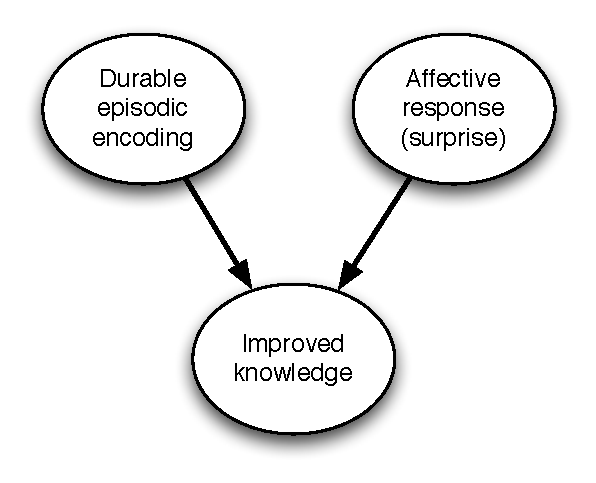
\includegraphics{causal1.pdf}
\end{center}
\caption{A graphical model representing the relationship between forms of
    psychological processing of factual information observed in
    chapter~\ref{chap:two}. Arrows represent conditional probability
    relationships and \emph{not necessarily causation}.}
\label{fig:causal-two}
\end{figure}
